\documentclass{standalone}
\usepackage{tikz}
\usetikzlibrary{positioning, fit, calc}
\begin{document}
    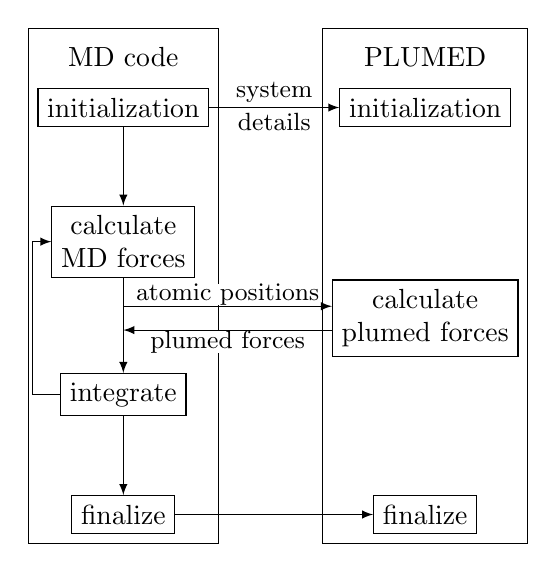
\begin{tikzpicture}
        \node[] (MD) {MD code};

        \node[below=1ex of MD, draw] (init){initialization};
        \node[below=of init, draw, align=center] (mdforces) {calculate\\MD forces};
        \node[below=8ex of mdforces, draw] (integrate) {integrate};
        \node[below=of integrate, draw] (finalize) {finalize};

        \node[fit=(MD)(init)(mdforces)(integrate)(finalize), draw] (MDblock) {};
        \draw[-latex] (init) -- (mdforces);
        \draw[-latex] (mdforces) -- (integrate);
        \draw[-latex] (integrate) -- (finalize);
        \draw[-latex] (integrate.west) -- ++ (-1em,0) |- (mdforces.west);

        \coordinate (a) at ($(mdforces)!.5!(integrate)$);

        \node[right=6em of MD] (plumed) {PLUMED};
        \node[below=of plumed] (b) {};

        \node[draw] (initplumed) at ($(plumed)!(init)!(b)$) {initialization};
        \node[draw, align=center] (plumedforces) at ($(plumed)!(a)!(b)$) {calculate\\plumed forces};
        \node[draw] (finalizeplumed) at ($(plumed)!(finalize)!(b)$) {finalize};

        \draw[-latex] (init) -- node[align=center, above=0.1ex, inner sep=0, outer sep=0, anchor=center] {\small system\\\small details} (initplumed);

        \coordinate (c) at ($(a)+(0,1ex)$);
        \draw[-latex] (c) -- node[above=0.1ex, align=center, inner sep=0, outer sep=0, fill=white] {\small atomic positions} (c-|plumedforces.west);

        \coordinate (d) at ($(a)+(0,-1ex)$);
        \draw[-latex] (plumedforces.west|-d) -- node[below=0.1ex, align=center, inner sep=0, outer sep=0, fill=white] {\small  plumed forces} (d);

        \draw[-latex] (finalize) -- (finalizeplumed);

        \node[fit=(plumed)(initplumed)(plumedforces)(finalizeplumed), draw] (plumedblock) {};
    \end{tikzpicture}
\end{document}
